\section{Problema}
\begin{frame}
	\frametitle{Problema} 
	\begin{exampleblock}{Pregunta investigaci�n}
	\justifying 
	\small �El \textit{conocimiento impl�cito} es un factor importante para la obtenci�n de \textit{recursos de informaci�n pertinentes} a una consulta?
	\end{exampleblock}
	
	\begin{figure}
	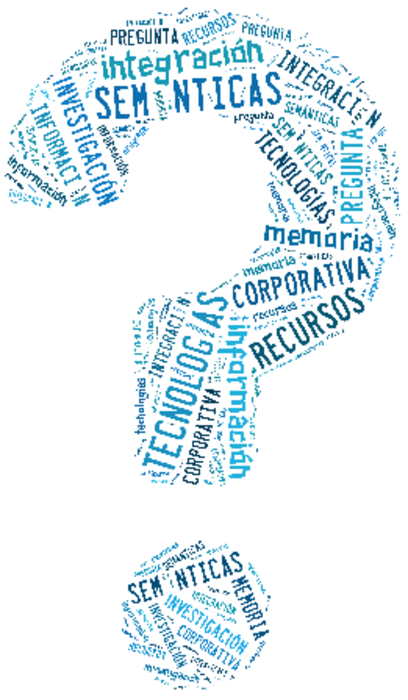
\includegraphics[scale=0.28]{PreguntaInv} 
	\end{figure}
	
	\begin{block}{Hip�tesis}
	\justifying 
	\small El uso de las \textit{tecnolog�as sem�nticas} es adecuado para lograr la \textit{integraci�n sem�ntica} de \textit{recursos de informaci�n} en una \textit{memoria corporativa}.
	\end{block}
\end{frame}

\subsection{Objetivo General}
\begin{frame}
	\frametitle{Objetivo General}
	\begin{alertblock}{}
	\justifying 
	Contribuir a la \textit{integraci�n sem�ntica} de los \textit{recursos de informaci�n} existentes en \textit{una memoria corporativa}, mediante el uso de las \textit{tecnolog�as sem�nticas}.
	\end{alertblock}
\end{frame}

\subsection{Objetivos}
\begin{frame}
	\frametitle{Objetivos Particulares} 
	\begin{enumerate}
	\item \justifying \small Proponer un \textbf{marco de referencia} para la \textit{integraci�n sem�ntica} de los \textit{recursos de informaci�n} existentes en una memoria corporativa.
	\item \justifying \small Proponer un \textbf{modelo sem�ntico} que represente el \textit{conocimiento expl�cito e impl�cito} existente en los \textit{recursos de informaci�n}.
	\item \justifying \small Implementar un \textbf{prototipo} que permita a los usuarios buscar y recuperar \textit{recursos de informaci�n} existentes en una memoria corporativa, as� como visualizar las caracterizaciones de estos recursos.
	\end{enumerate}
\end{frame}

%\subsection{Metodolog�a}
%\begin{frame}
%	\frametitle{Metodolog�a I}
%	\begin{block}{Marco de Referencia}
%	\begin{enumerate}
%	\item \justifying \small Identificar los principales \textit{casos de uso}.
%	\item \justifying \small Evaluar las \textit{herramientas sem�nticas}.
%	\item \justifying \small Componer la \textit{memoria corporativa} de RyT.
%	\end{enumerate}
%	
%	\begin{exampleblock}{Modelo Sem�ntico}
%	\begin{enumerate}
%	\setcounter{enumi}{3}
%	\item \justifying \small Representar el \textit{conocimiento expl�cito} de los \textit{recursos de informaci�n} en un \textit{modelo sem�ntico} (ontolog�a).
%	\item \justifying \small Enriquecer el \textit{modelo sem�ntico} con \textit{reglas de inferencia}.
%	\end{enumerate}
%	\end{exampleblock}
%	
%	\begin{enumerate}
%	\setcounter{enumi}{5}
%	\item \justifying \small Encontrar las principales \textit{consultas}.
%	\item \justifying \small Hacer expl�cito el conocimiento impl�cito.
%	\item \justifying \small Buscar y recuperar informaci�n en el modelo inferido.
%	\end{enumerate}
%	\end{block}
%\end{frame}
%
%\begin{frame}
%	\frametitle{Metodolog�a II}	
%	\begin{block}{Prototipo de interfaz gr�fica de usuario}	
%	\begin{enumerate}
%	\setcounter{enumi}{8}
%	\item \justifying \small Construir el \textit{prototipo de interfaz de usuario} para la (b�squeda y navegaci�n) de los usuarios en un modelo sem�ntico.
%	\end{enumerate}
%	\end{block}
%	
%	\begin{block}{Evaluaci�n}
%	\begin{enumerate}
%	\setcounter{enumi}{9}
%	\item \justifying \small Evaluar la calidad de los resultados con y sin inferencia.
%	\item \justifying \small Evaluar los \textit{tiempos promedios} de consulta sobre modelos con/sin inferencia.
%	\end{enumerate}
%	\end{block}
%\end{frame}
